\chapter{Opis projektnog zadatka}
		
		
    		Ovaj je projektni zadatak baziran na temi doniranja krvi. Ovom se aplikacijom doniranje   krvi nastoji automatizirati i dodatno olakšati te približiti potencijalnim donorima, ali i osobama koje dosad nisu donirale krvi te na taj način poboljšali sveukupno stanje i zalihe krvi. Na taj će se način automatizirati organiziranje doniranja krvi što će rezultirati boljom situacijom za kritične slučajeve. 
        	Prilikom samog pokretanja aplikacije, prikazat će se dostupna mjesta za doniranje krvi. Korisniku koji se nije registrirao, a želi vidjeti dostupna mjesta za doniranje krvi, bit će omogućeno tako što će se, odabirom na željeno mjesto, prikazati datum, mjesto i vrijeme organiziranih akcija doniranja krvi. Nadalje, neregistriranom korisniku bit će dostupne informacije o trenutno potrebnoj krvnoj grupi za odabrano mjesto. Korisniki koji se želi prijaviti u sustav bit će omogućeno prijaviti se s postojećim računom, uz pretpostavku da ga korisnik posjeduje, ili kreiranjem novog korisničkog računa za što će mu biti potrebno unijeti sljedeće podatke:
		\begin{packed_item}
			\item \textit{korisničko ime}
			\item \textit{lozinka}
			\item \textit{ime i prezime osobe}
			\item \textit{OIB}
			\item \textit{adresa}
			\item \textit{broj mobitela}
			\item \textit{email adresa osobe}
		\end{packed_item}
		
    		Registracijom korisnika u sustav, korisnik postaje potencijalni donor krvi. Nakon registracije, potencijalni donor može odabrati željenu lokaciju i rezervirati termin doniranja. Prije same rezervacije termina doniranja, korisnik mora potvrditi sustavu da se slaže s verificiranjem kritičnih podataka uporabom središnjeg informacijskog sustava primarne zdravstvene zaštite RH.\\
            \textbf{Donor} odabirom krvne grupe filtrira mjesta za doniranje krvi, prema potrebi, te na taj način popunjuje, odnosno rezervira, slobodno mjesto za doniranje. Nakon odlaska na mjesto doniranja krvi, korisnik se uvodi u evidenciju koja mu je dostupna u sustavu u bilo kojem trenutku. U slučaju da nema slobodnih mjesta za odabranu lokaciju doniranja krvi, sustav će pravovremeno obavijestiti korisnika te mu ponuditi alternativne lokacije. Osoba nije obvezna doći na rezerviran termin donacije krvi, međutim, popunjavanjem mjesta za doniranje krvi oduzima se mjesto potencijalnom donoru. Osoba u svakom trenutku može otkazati rezervaciju. Korisniku će na vrijeme biti poslan podsjetnik/obavijest kako bi na vrijeme mogao doći na termin ili kako bi znao postoji li potreba za donacijom. Registrirani korisnik može u svakom trenutku vidjeti svoju povijest doniranja kao i svoju medicinsku povijest.\\
            \textbf{Administrator} sustava verificira kritične podatke uporabom središnjeg informacijskog sustava primarne zdravstvene zaštite RH. Uloga je administratora administriranje stranice i registriranih korisnika kao i upravljanje bazom podataka te podacima samih korisnika. Administrator ima mogućnost ažuriranja lokacija za doniranje krvi, pristup povijesti donacija za svakog korisnika kao i pristup kritičnim podacima koje korisnik mora potvrditi. \\
            \textbf{Organizacije za prikupljanje krvi} redovito ažuriraju podatke o dostupnim zalihama krvi u svojim centrima putem aplikacije kako bi korisnici mogli vidjeti trenutnu dostupnost krvnih grupa. Osim toga, unose podatke i informacije o svojim centrima za darivanje krvi putem aplikacije što uključuje lokacije, radnom vremenu, kontaktu i slično. Također, organizacije mogu koristiti aplikaciju za komunikaciju s donatorima putem obavijesti o hitnim potrebama, podsjetnicima na donacije i zahvalama za njihovu podršku, a uz to mogu i planirati i organizirati donacije i promocije donatora.\\


            Dodat će se još naknadno s daljnom implementacijom
		\eject
		
		\section{IZBRISATI}
		
		\textit{Ovo potpoglavlje izbrisati.}\\

		U nastavku se nalaze različiti primjeri kako koristiti osnovne funkcionalnosti \LaTeX a koje su potrebne za izradu dokumentacije. Za dodatnu pomoć obratiti se asistentu na projektu ili potražiti upute na sljedećim web sjedištima:
		\begin{itemize}
			\item Upute za izradu diplomskog rada u \LaTeX u - \url{https://www.fer.unizg.hr/_download/repository/LaTeX-upute.pdf}
			\item \LaTeX\ projekt - \url{https://www.latex-project.org/help/}
			\item StackExchange za Tex - \url{https://tex.stackexchange.com/}\\
		
		\end{itemize} 	


		
		\noindent \underbar{podcrtani tekst}, \textbf{podebljani tekst}, 	\textit{nagnuti tekst}\\
		\noindent \normalsize primjer \large primjer \Large primjer \LARGE {primjer} \huge {primjer} \Huge primjer \normalsize
				
		\begin{packed_item}
			
			\item  primjer
			\item  primjer
			\item  primjer
			\item[] \begin{packed_enum}
				\item primjer
				\item[] \begin{packed_enum}
					\item[1.a] primjer
					\item[b] primjer
				\end{packed_enum}
				\item primjer
			\end{packed_enum}
			
		\end{packed_item}
		
		\noindent primjer url-a: \url{https://www.fer.unizg.hr/predmet/proinz/projekt}
		
		\noindent posebni znakovi: \# \$ \% \& \{ \} \_ 
		$|$ $<$ $>$ 
		\^{} 
		\~{} 
		$\backslash$ 
		
		
		\begin{longtblr}[
			label=none,
			entry=none
			]{
				width = \textwidth,
				colspec={|X[8,l]|X[8, l]|X[16, l]|}, 
				rowhead = 1,
			} %definicija širine tablice, širine stupaca, poravnanje i broja redaka naslova tablice
			\hline \SetCell[c=3]{c}{\textbf{naslov unutar tablice}}	 \\ \hline[3pt]
			\SetCell{LightGreen}IDKorisnik & INT	&  	Lorem ipsum dolor sit amet, consectetur adipiscing elit, sed do eiusmod  	\\ \hline
			korisnickoIme	& VARCHAR &   	\\ \hline 
			email & VARCHAR &   \\ \hline 
			ime & VARCHAR	&  		\\ \hline 
			\SetCell{LightBlue} primjer	& VARCHAR &   	\\ \hline 
		\end{longtblr}
		

		\begin{longtblr}[
				caption = {Naslov s referencom izvan tablice},
				entry = {Short Caption},
			]{
				width = \textwidth, 
				colspec = {|X[8,l]|X[8,l]|X[16,l]|}, 
				rowhead = 1,
			}
			\hline
			\SetCell{LightGreen}IDKorisnik & INT	&  	Lorem ipsum dolor sit amet, consectetur adipiscing elit, sed do eiusmod  	\\ \hline
			korisnickoIme	& VARCHAR &   	\\ \hline 
			email & VARCHAR &   \\ \hline 
			ime & VARCHAR	&  		\\ \hline 
			\SetCell{LightBlue} primjer	& VARCHAR &   	\\ \hline 
		\end{longtblr}
	


		
		
		%unos slike
		\begin{figure}[H]
			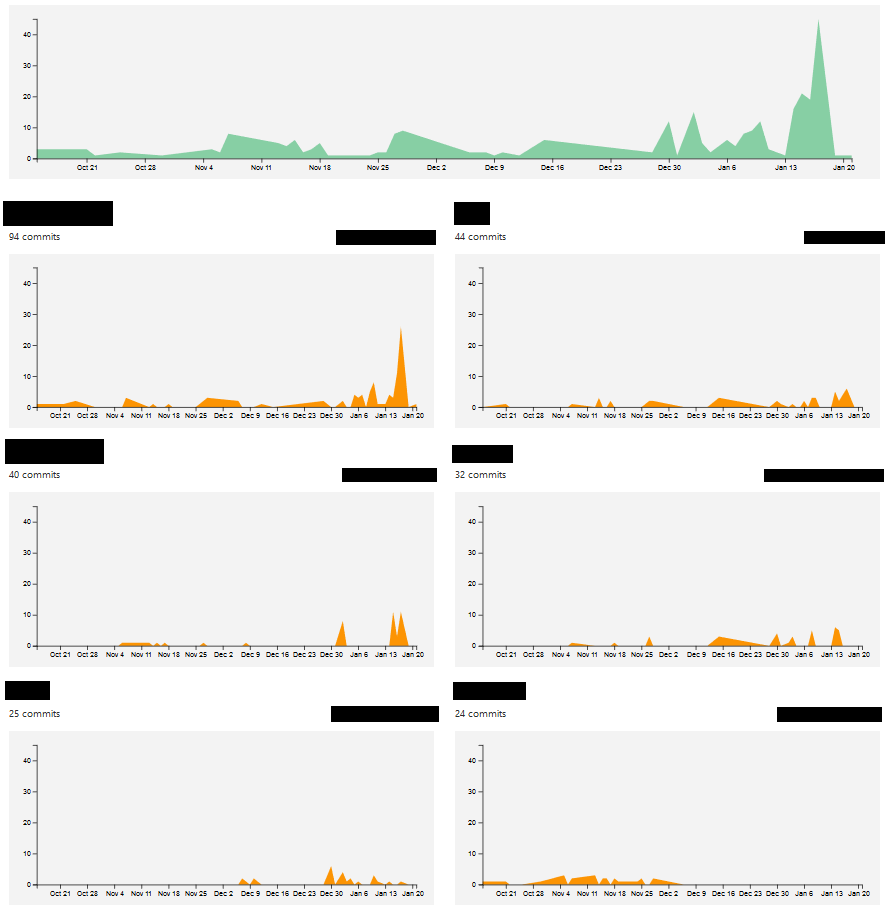
\includegraphics[scale=0.4]{slike/aktivnost.PNG} %veličina slike u odnosu na originalnu datoteku i pozicija slike
			\centering
			\caption{Primjer slike s potpisom}
			\label{fig:promjene}
		\end{figure}
		
		\begin{figure}[H]
			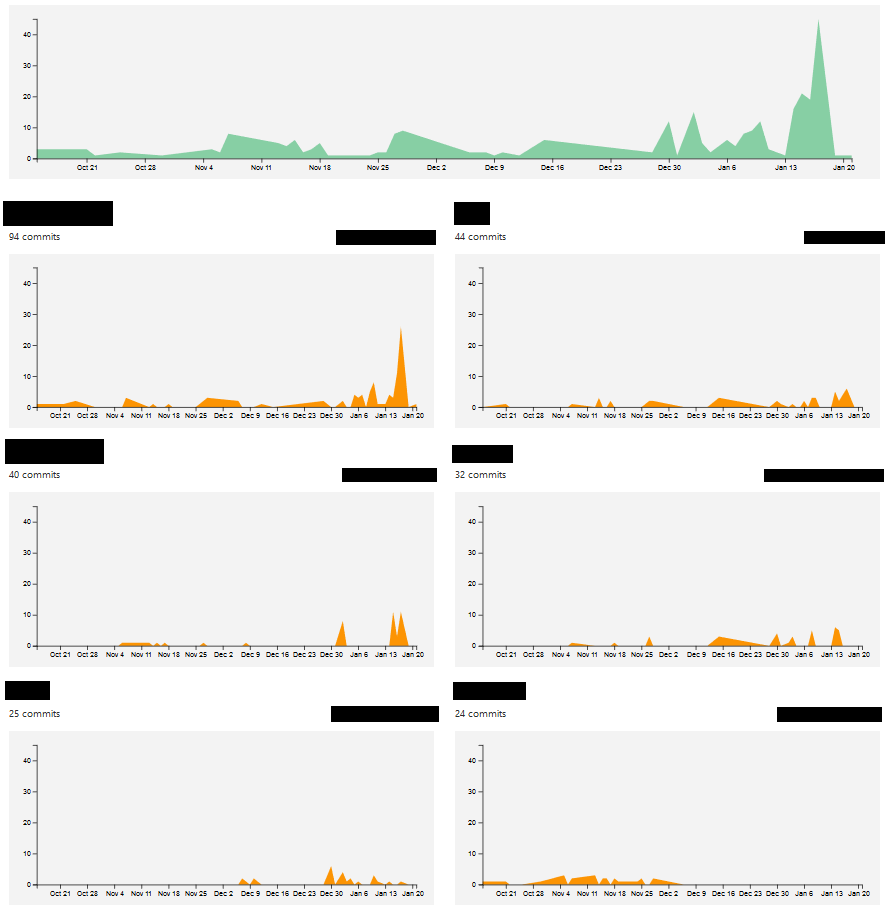
\includegraphics[width=\textwidth]{slike/aktivnost.PNG} %veličina u odnosu na širinu linije
			\caption{Primjer slike s potpisom 2}
			\label{fig:promjene2} %label mora biti drugaciji za svaku sliku
		\end{figure}
		
		Referenciranje slike \ref{fig:promjene2} u tekstu.
		
		\eject
		
	